\documentclass{article}
\usepackage{fancyhdr}
\usepackage{datetime}
\usepackage{parskip}
\usepackage{graphicx}

\newdateformat{monthyeardate}{\monthname[\THEMONTH], \THEYEAR}

\pagestyle{fancy}

\fancyhf{}
\fancyfoot[L]{University of Oulu. \monthyeardate\today}

\lhead{IoT Data Analytics}
\rhead{Page \thepage}

\title{
Exercise 3: Small IoT Implementation
\bigskip
\author{Andrei Golubev 2621924 \\ Hassan Shaheen 2600602}
\date{\parbox{\linewidth}{\centering
  \endgraf\bigskip
  University of Oulu, Oulu, Finland
  \endgraf\monthyeardate\today}}
}

\setlength{\parindent}{0pt}

\begin{document}
\maketitle
\thispagestyle{empty}
\newpage

\section{Description of design}

In this exercise we design a simple device-to-device communication system that allows one device to
control another in a certain way. Specifically, we focus on a remote control of PC's keyboard by
virtualizing a small subset of keyboard events ("key press", "key release"). Our implementation, yet
limited, can further be generalized to any remote control functionality as the approach is generic
in its core.

Thus, the idea is to control a nearby computer/laptop remotely using an Android application. For
this purpose, a \textbf{Bluetooth remote controller} is implemented that establishes a connection
with a Windows PC running a server-side script (listener). We focus on limited media control keys
that allow us to seamlessly control applications that support media keyboard inputs, for example,
Spotify or YouTube.

\subsection{Objective}

The objective of this application is that the Android device can work as a \textbf{generic remote
controller} for a computer. Even though in current application users can only control limited media
options, it can be used in things like controlling the mouse with touchpad, changing the volume of
the PC, controlling slide shows, etc. The main purpose is to control your PC remotely and, depending
on the need, it can be used by students for their presentations or by a regular person who just
wants to change their laptop music without getting up.

\subsection{Design}
The system has two parts an Android application with a controller interface and a server application
running on windows which interprets the commands sent from the device.

\subsubsection{Android Application}
The flow of the Android application is the following (the pictures for different stages can be seen
below).

\begin{enumerate}
\item Users will search for Bluetooth devices

\begin{figure}[ht]
\centering
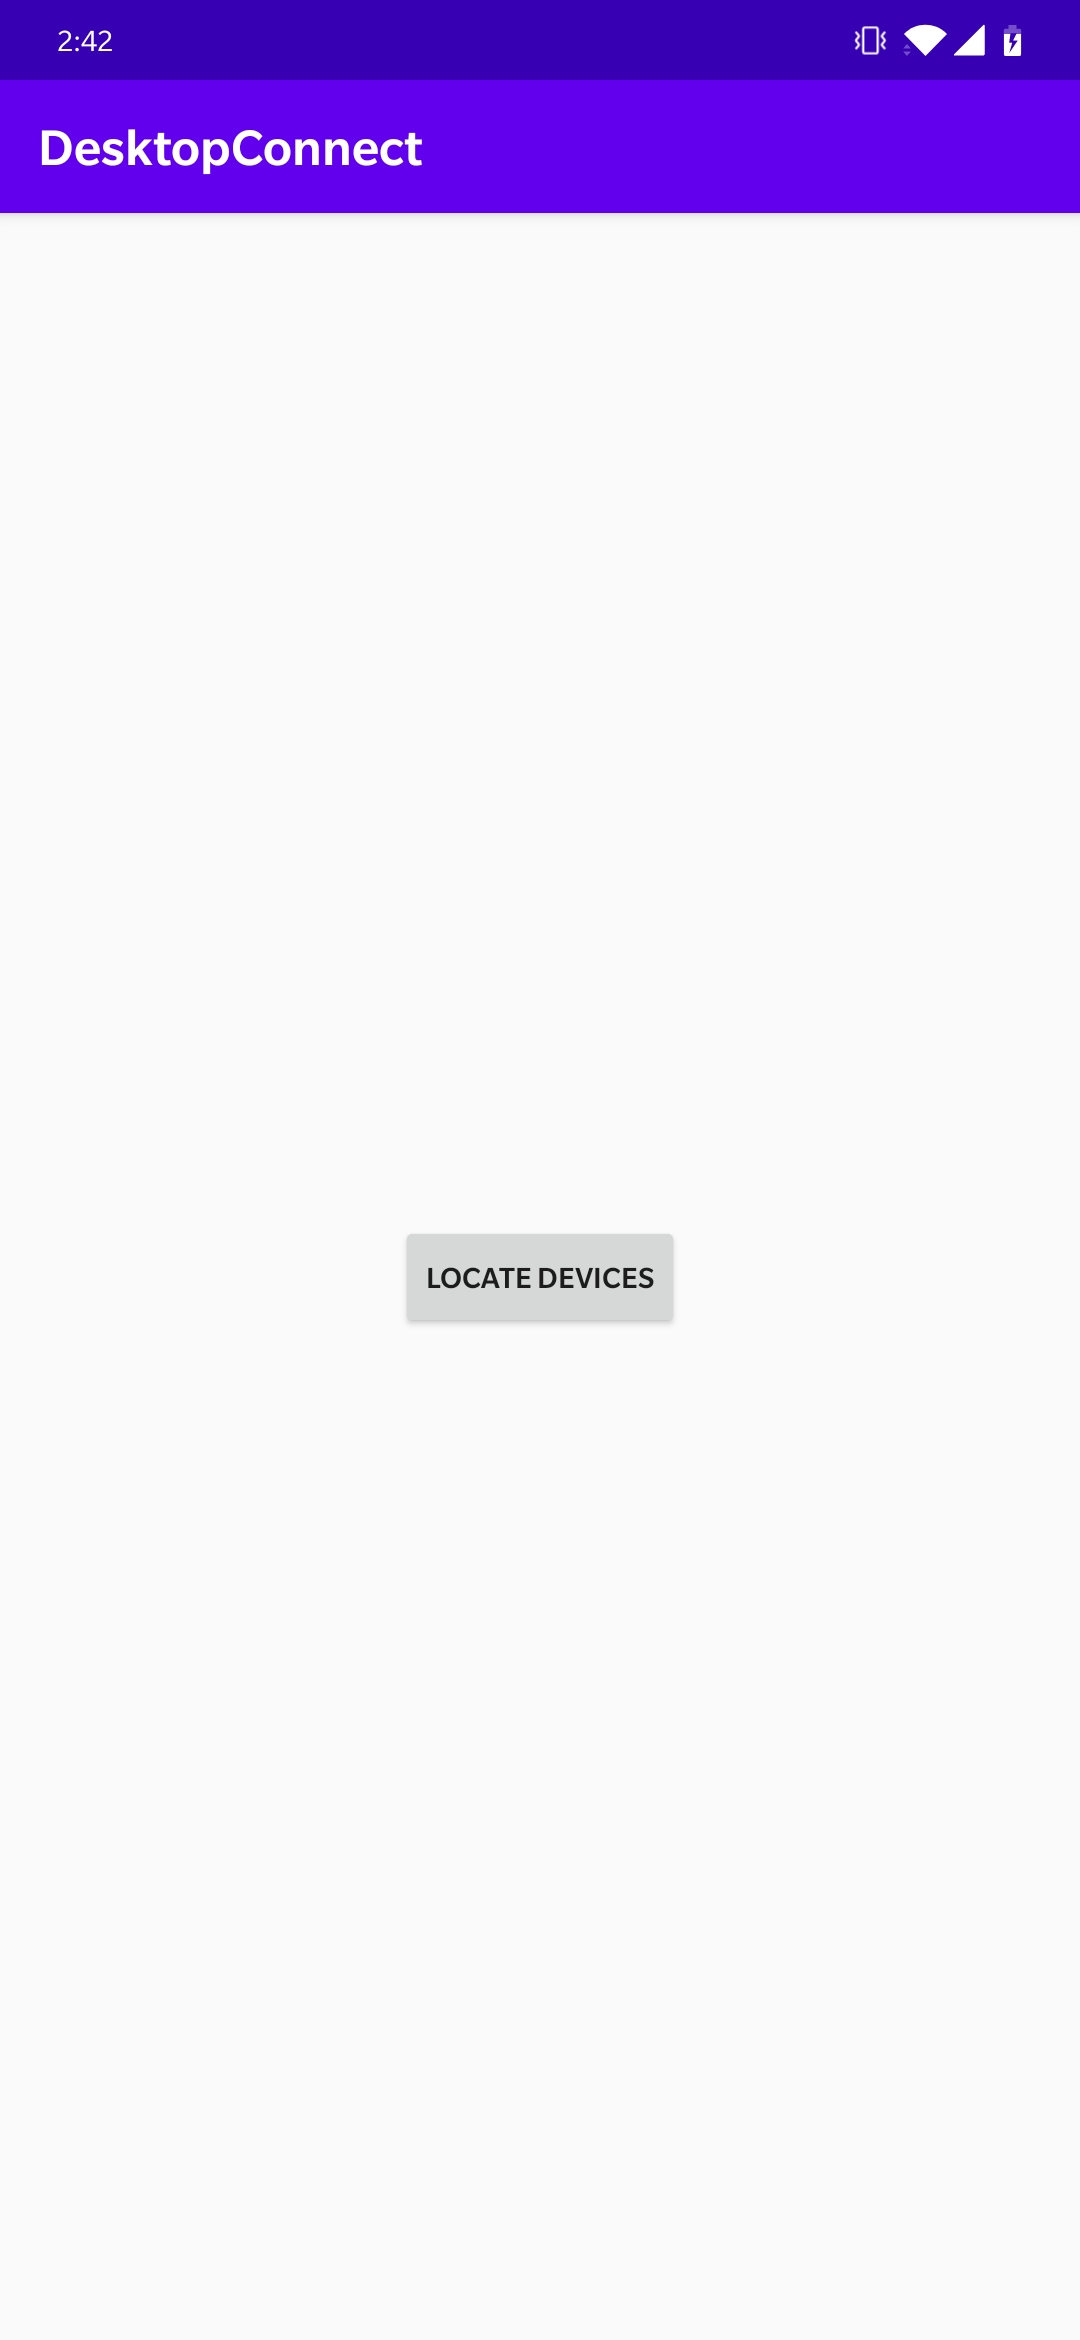
\includegraphics[width=90mm]{./locate.jpg}
\end{figure}

\item To locate, the user needs to make the device discoverable,  after successful discovery, the
application will show the list of two kinds of devices, Ones who are already been paired or are
available.

\begin{figure}[ht]
\centering
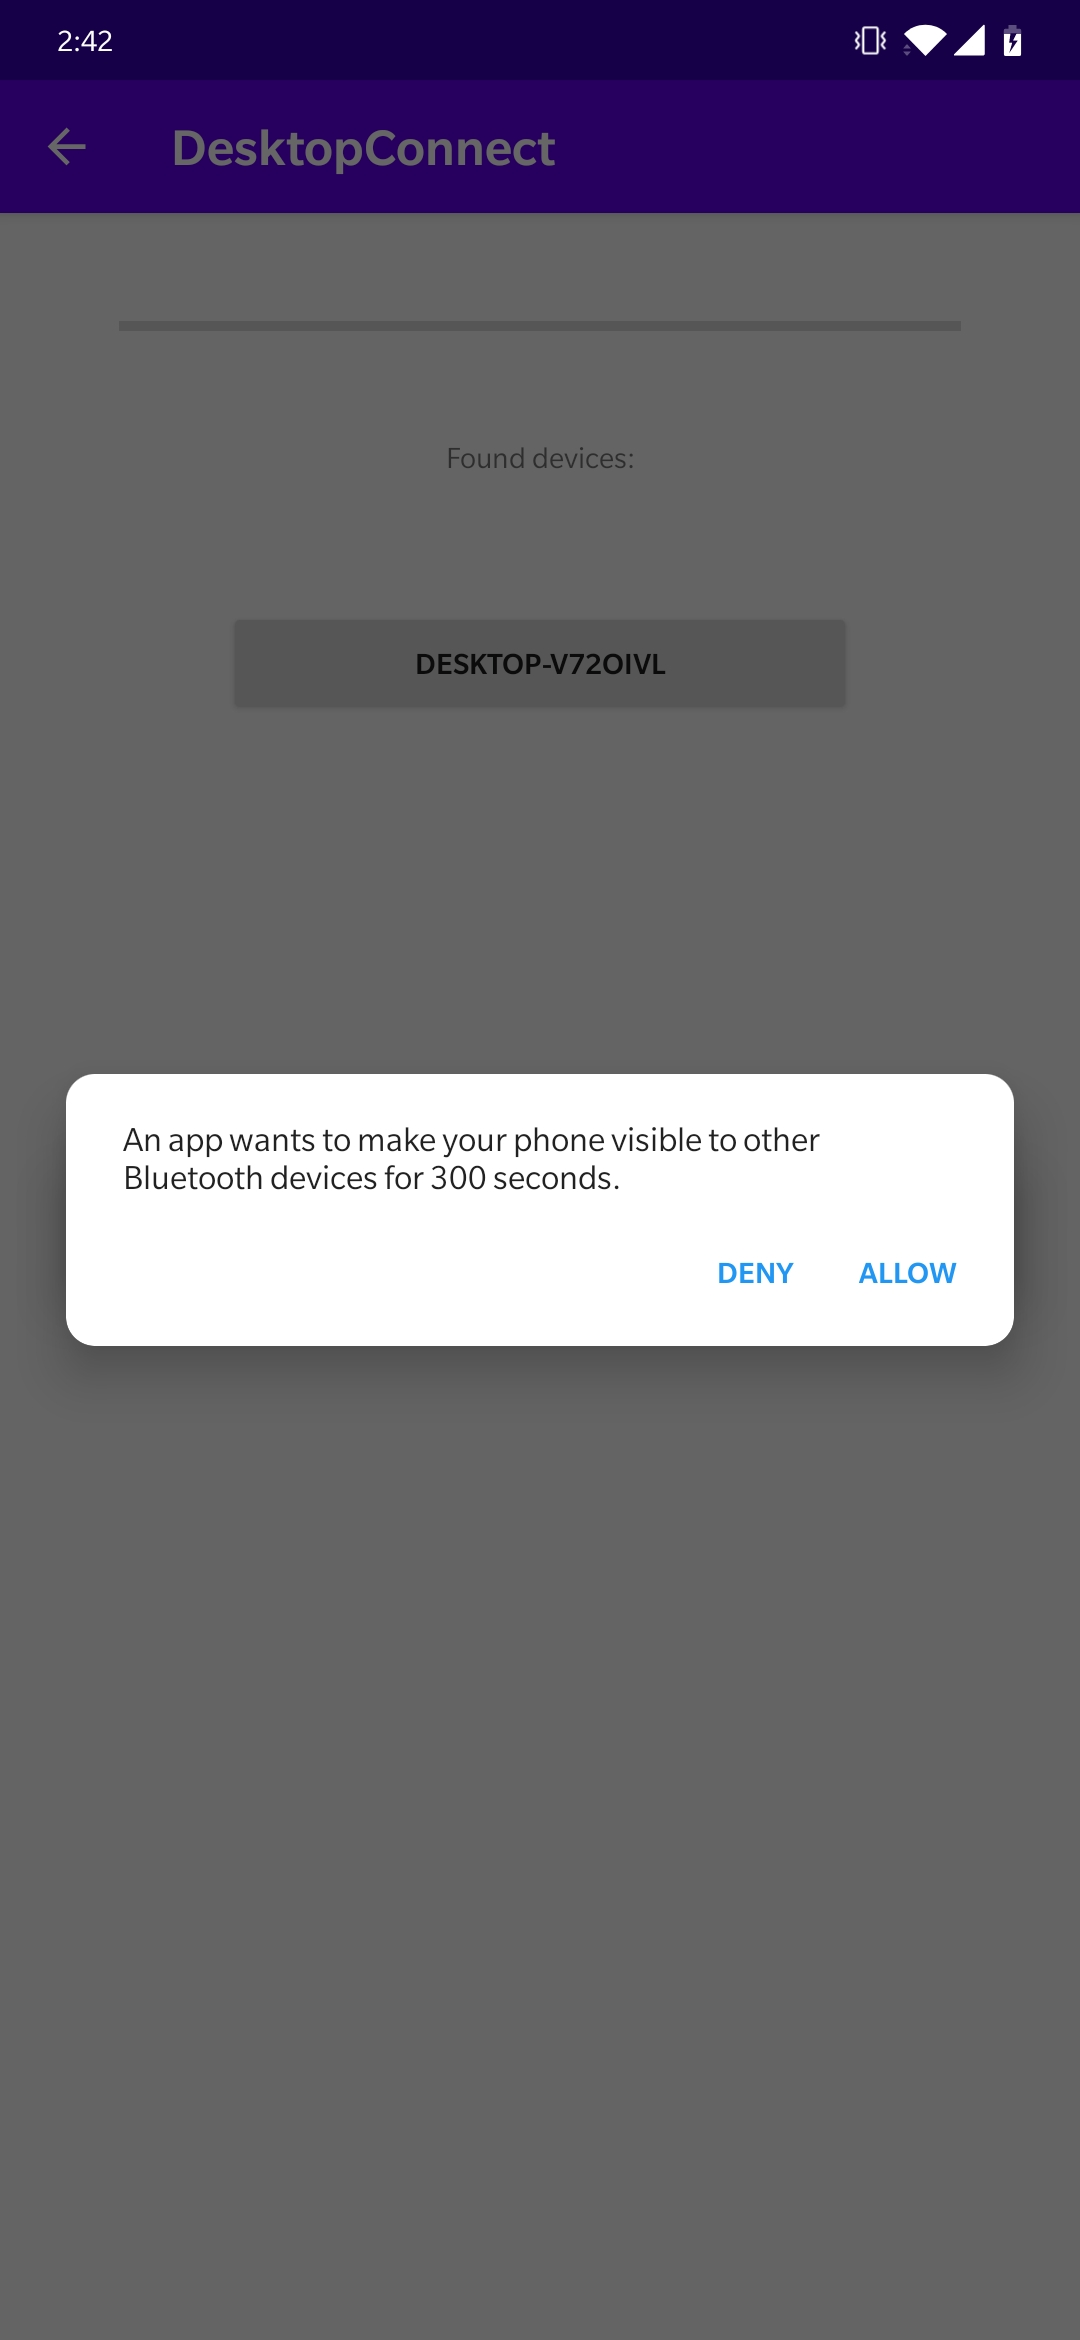
\includegraphics[width=90mm]{./discover.jpg}
\end{figure}

\item User can select his/her computer and the application will connect with the server running on
windows. The next screen will show four types of controls by pressing these buttons user sends the
commands to the computer.
\begin{itemize}
\item Play/Pause
\item Next
\item Previous
\item Stop
\end{itemize}

\begin{figure}[ht]
\centering
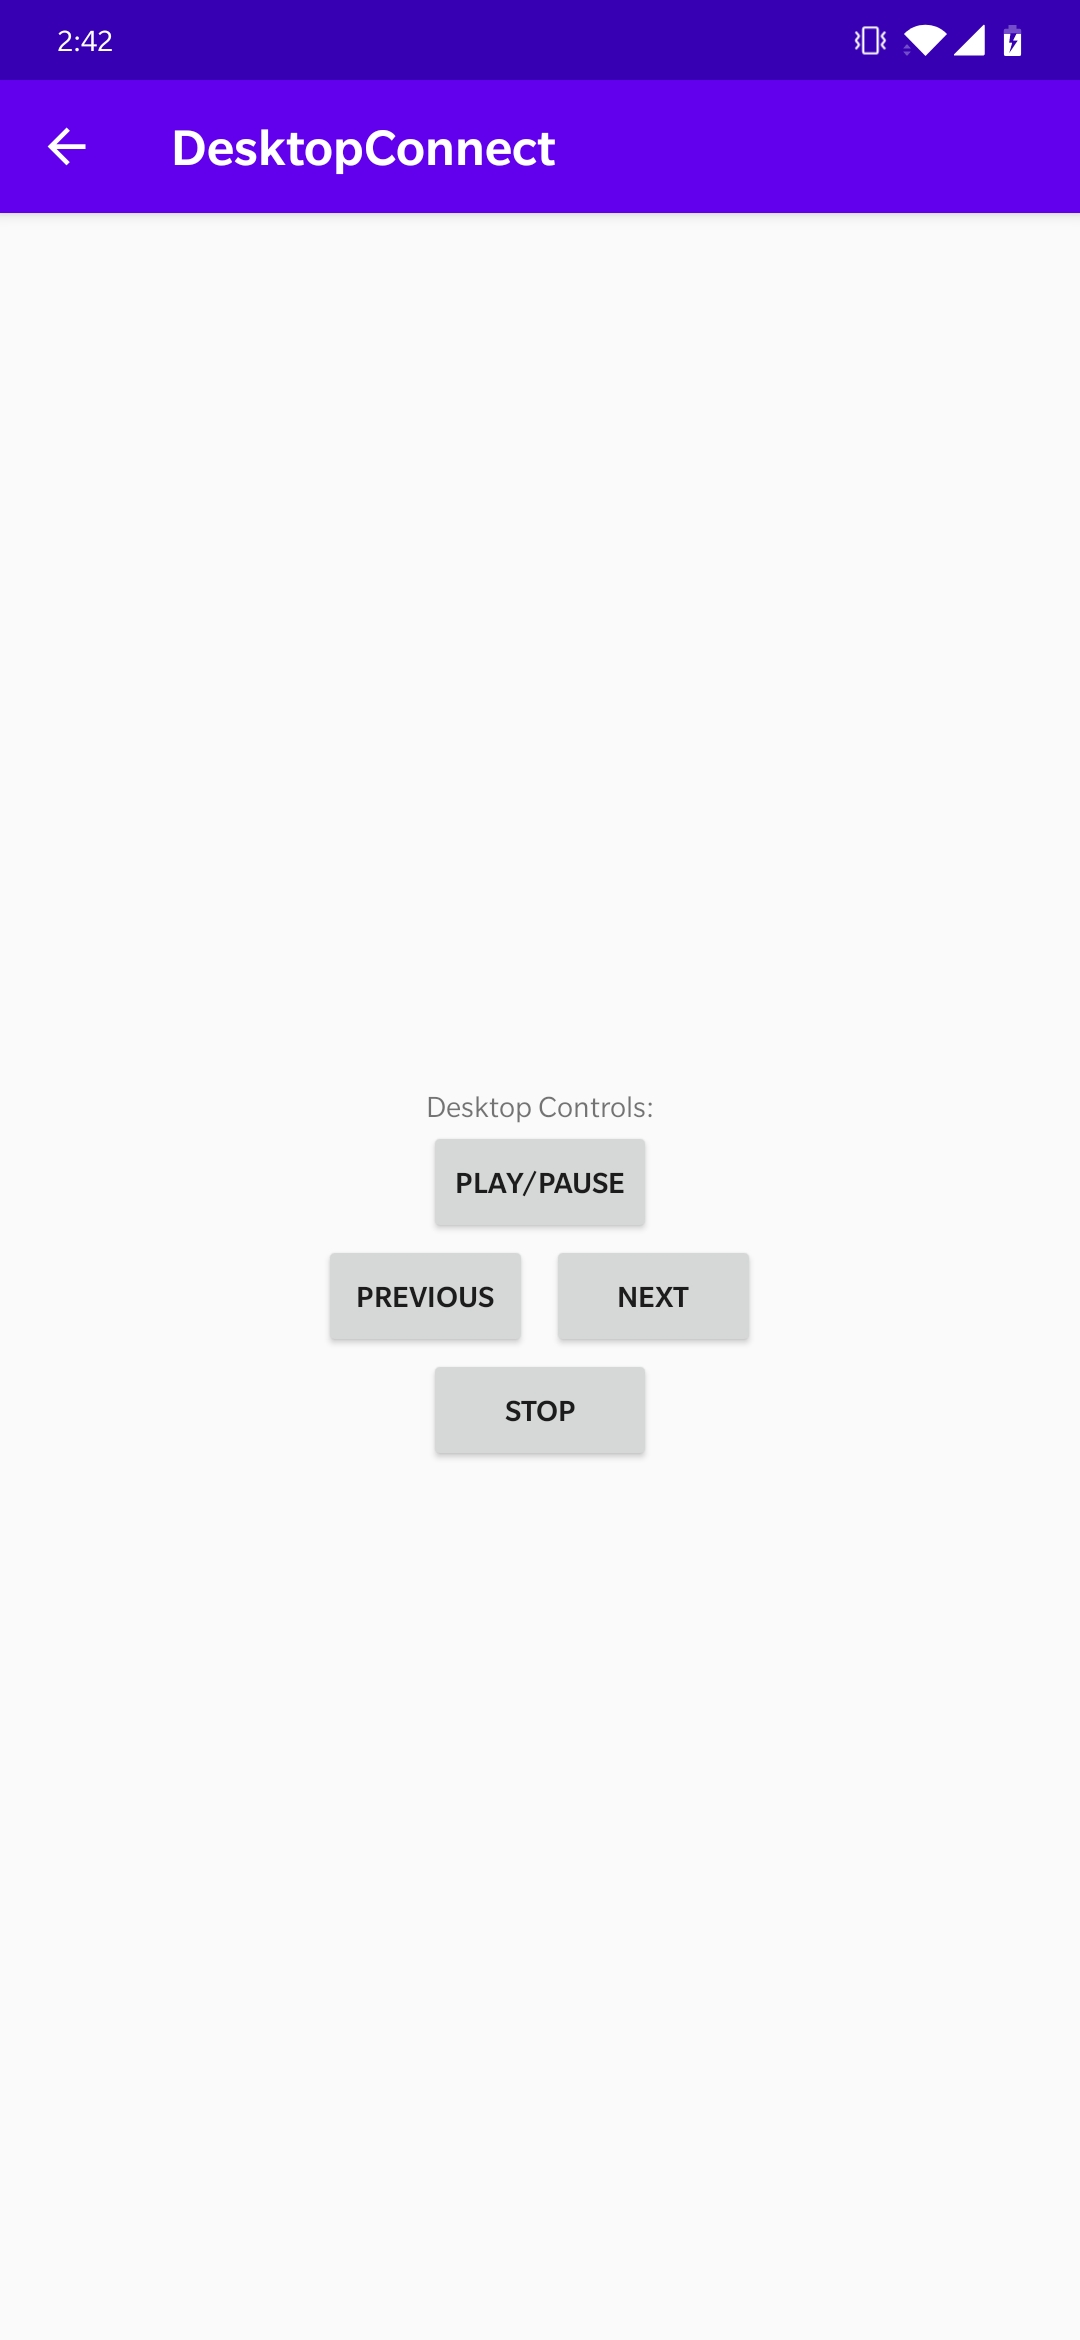
\includegraphics[width=90mm]{./control.jpg}
\end{figure}

\end{enumerate}


\subsubsection{Server side}
The Windows PC being a server will receive these commands from Android device and interpret them
accordingly. The user can see which Android device is connected and what commands are being sent.

\begin{figure}[ht]
\centering
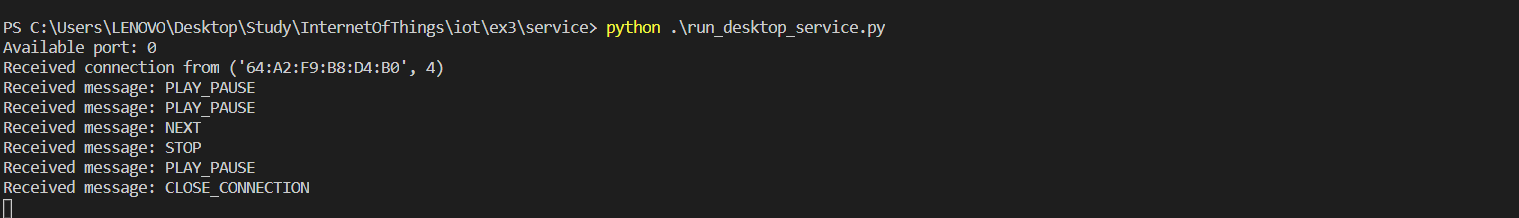
\includegraphics[scale=.3]{./service.png}
\end{figure}

\section{Technical Implementation}

\subsection{Android Application}

For the Android application, we are using its Bluetooth library. For Bluetooth-enabled devices to
transmit data between each other, they must first form a channel of communication using a pairing
process.

To use Bluetooth features in our application we need mainly two permissions
android.permission.\textbf{BLUETOOTH} and android.permission.\textbf{ACCESS\textunderscore FINE
\textunderscore LOCATION}. We prompt the user if any of these permissions are missing. If not, we
start the discovery process. There are two parts, we show the list of already paired devices or
start the discovery of available devices using a class named \textbf{BluetoothAdapter}.

\begin{figure}[ht]
\centering
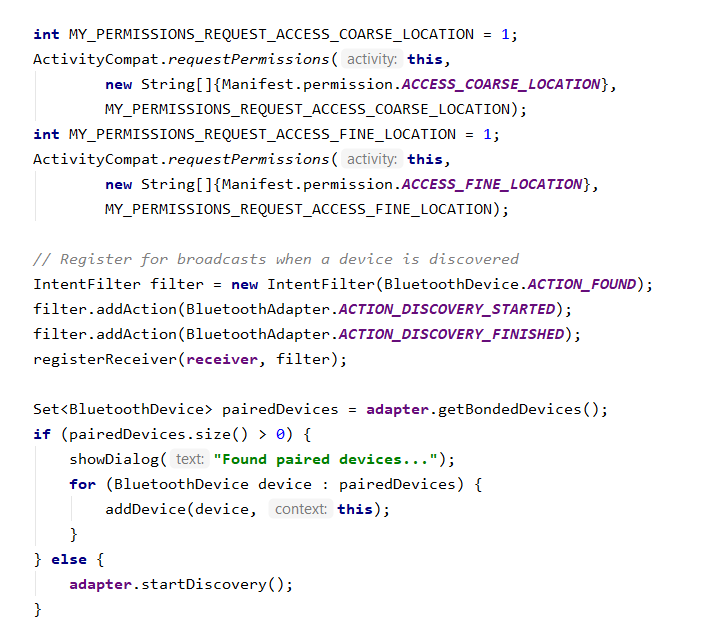
\includegraphics[width=90mm]{./discoverDevice.png}
\end{figure}


After we have our device we can connect to the socket on the computer/laptop running our server
using the same \textbf{UUID} we have it on our server.  For sending commands we have buttons that
invoke an event with commands when they are clicked.

For example, when “PLAY/PAUSE” button is clicked. It will invoke \textbf{SendMessage()} function
with the string “PLAY/PAUSE” as a parameter which is then sent to the server and executed.

\begin{figure}[ht]
\centering
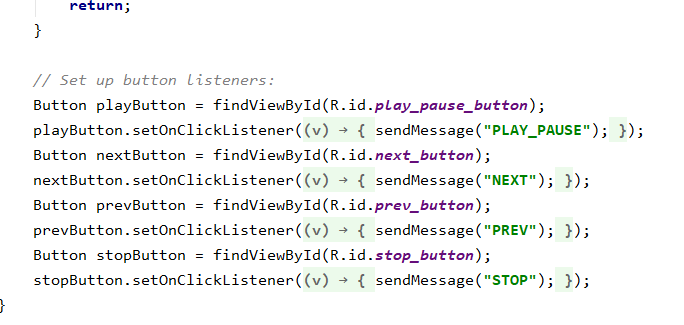
\includegraphics[width=90mm]{./sendMsg.png}
\end{figure}

\subsection{Windows Server side}

For our Windows PC, we are using \textbf{Python}. There are two main libraries used in this project:

\begin{itemize}
\item \textbf{Pynput} allows controlling the input devices, in our case a computer keyboard

\item \textbf{PyBluez} helps python code to access the host machine Bluetooth resources
\end{itemize}

Communication is done using a socket programming model, a socket represents an endpoint of a
communication channel. The first step is to establish a connection using a socket. For that, we need
a protocol for the socket in our case its \textbf{RFCOMM}. After binding the socket with an
available port, we start advertising over Bluetooth.

The method we are using is \textbf{Bluetooth.advertise\textunderscore service(socket, UUID)} this
method takes a socket and UUID. It looks for service with the same UUID to connect (our android
application).

After the connection is made, we are receiving messages on this port. The messages are in a
predefined string format. Which are then converted to windows virtual keycodes and interpreted in
keyboard commands using \textbf{Pynput}.

\begin{figure}[ht]
\centering
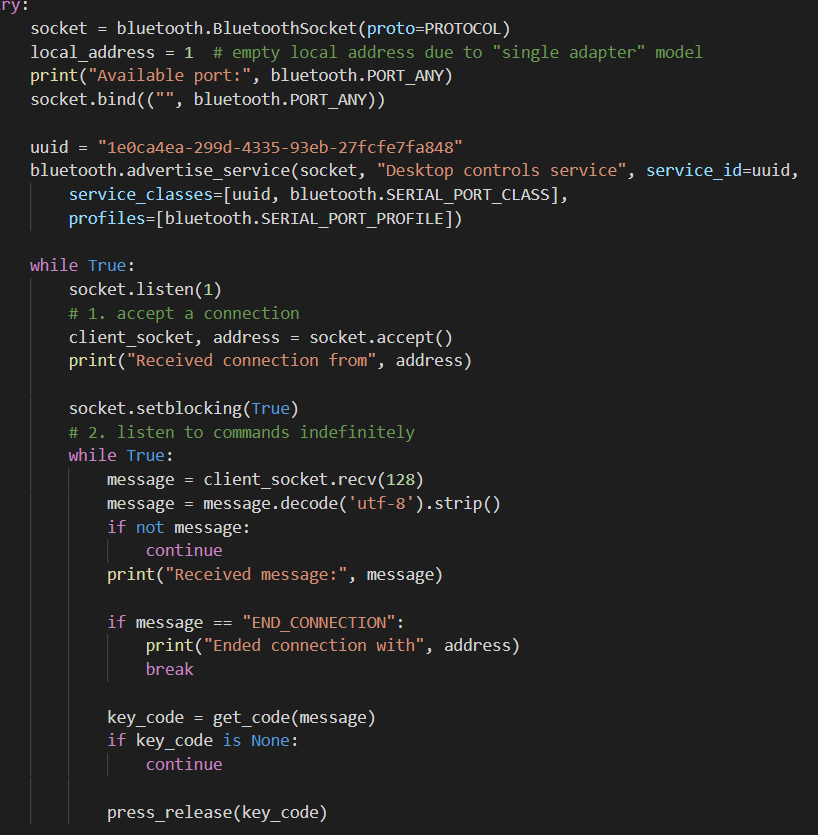
\includegraphics[width=90mm]{./socket.png}
\end{figure}

For example, if the user presses PLAY/PAUSE in an Android application, a string is received on the
server, gets converted to Windows keycode for PLAY/PAUSE, and then executed using Pynput keyboard
controller.


\section{References}

1. Pynput library. URL: https://pypi.org/project/pynput/

2. PyBluez project. URL: https://github.com/pybluez/pybluez

3. Android Bluetooth. URL: https://developer.android.com/guide/topics/connectivity/bluetooth

\end{document}
